% -----------------------------------Initialize Document----------------------------------------
\documentclass[12pt]{article}
\usepackage{textcomp}
\usepackage[headheight=12pt, headsep=0pt, nohead, nofoot]{geometry}
\usepackage{graphicx}
\usepackage{subfig}
\usepackage{multicol}
\usepackage{siunitx}
\usepackage{wrapfig}
\setlength{\footskip}{40pt}

\DeclareSIUnit\gauss{G}
\usepackage[utf8x]{inputenc}
\usepackage[british,UKenglish]{babel}
\usepackage{amsmath}
%\usepackage{titlesec}
\usepackage{color}
\usepackage{graphicx}
\usepackage{fancyref}
\usepackage{hyperref}
\usepackage{float}
\usepackage{scrextend}
\usepackage{setspace}
\usepackage{xargs}
\usepackage{multicol}
\usepackage{nameref}
\usepackage[pdftex,dvipsnames]{xcolor}
\usepackage{sectsty}
\usepackage{multicol}
\usepackage{multirow}
\usepackage[procnames]{listings}
\usepackage{appendix}
\usepackage{cite}

\newcommand\tab[1][1cm]{\hspace*{#1}}
\hypersetup{colorlinks=true, linkcolor=black}
\interfootnotelinepenalty=10000
%\titleformat*{\subsubsection}{\large\bfseries}
%\subsubsectionfont{\large}
%\subsectionfont{\Large}
%\sectionfont{\LARGE}
\definecolor{cleanOrange}{HTML}{D14D00}
\definecolor{cleanYellow}{HTML}{FFFF99}
\definecolor{cleanBlue}{HTML}{3d0099}
%\newcommand{\cleancode}[1]{\begin{addmargin}[3em]{3em}\fcolorbox{cleanOrange}{cleanYellow}{\texttt{\textcolor{cleanOrange}{#1}}}\end{addmargin}}
\newcommand{\cleancode}[1]{\begin{addmargin}[3em]{3em}\texttt{\textcolor{cleanOrange}{#1}}\end{addmargin}}
\newcommand{\cleanstyle}[1]{\text{\textcolor{cleanOrange}{\texttt{#1}}}}


\usepackage[colorinlistoftodos,prependcaption,textsize=footnotesize]{todonotes}
\newcommandx{\commred}[2][1=]{\textcolor{Red}
{\todo[linecolor=red,backgroundcolor=red!25,bordercolor=red,#1]{#2}}}
\newcommandx{\commblue}[2][1=]{\textcolor{Blue}
{\todo[linecolor=blue,backgroundcolor=blue!25,bordercolor=blue,#1]{#2}}}
\newcommandx{\commgreen}[2][1=]{\textcolor{OliveGreen}{\todo[linecolor=OliveGreen,backgroundcolor=OliveGreen!25,bordercolor=OliveGreen,#1]{#2}}}
\newcommandx{\commpurp}[2][1=]{\textcolor{Plum}{\todo[linecolor=Plum,backgroundcolor=Plum!25,bordercolor=Plum,#1]{#2}}}

\def\code#1{{\tt #1}}

\def\note#1{\noindent{\bf [Note: #1]}}

\makeatletter
%% The "\@seccntformat" command is an auxiliary command
%% (see pp. 26f. of 'The LaTeX Companion,' 2nd. ed.)
\def\@seccntformat#1{\@ifundefined{#1@cntformat}%
   {\csname the#1\endcsname\quad}  % default
   {\csname #1@cntformat\endcsname}% enable individual control
}
\let\oldappendix\appendix %% save current definition of \appendix
\renewcommand\appendix{%
    \oldappendix
    \newcommand{\section@cntformat}{\appendixname~\thesection\quad}
}
\makeatother
% "define" Scala
\usepackage[T1]{fontenc}  
\usepackage[scaled=0.82]{beramono}  
\usepackage{microtype} 

\sbox0{\small\ttfamily A}
\edef\mybasewidth{\the\wd0 }

\lstdefinelanguage{scala}{
  morekeywords={abstract,case,catch,class,def,%
    do,else,extends,false,final,finally,%
    for,if,implicit,import,match,mixin,%
    new,null,object,override,package,%
    private,protected,requires,return,sealed,%
    super,this,throw,trait,true,try,%
    type,val,var,while,with,yield},
  sensitive=true,
  morecomment=[l]{//},
  morecomment=[n]{/*}{*/},
  morestring=[b]",
  morestring=[b]',
  morestring=[b]"""
}

\usepackage{color}
\definecolor{dkgreen}{rgb}{0,0.6,0}
\definecolor{gray}{rgb}{0.5,0.5,0.5}
\definecolor{mauve}{rgb}{0.58,0,0.82}

% Default settings for code listings
\lstset{frame=tb,
  language=scala,
  aboveskip=3mm,
  belowskip=3mm,
  showstringspaces=false,
  columns=fixed, % basewidth=\mybasewidth,
  basicstyle={\small\ttfamily},
  numbers=none,
  numberstyle=\footnotesize\color{gray},
  % identifierstyle=\color{red},
  keywordstyle=\color{blue},
  commentstyle=\color{dkgreen},
  stringstyle=\color{mauve},
  frame=single,
  breaklines=true,
  breakatwhitespace=true,
  procnamekeys={def, val, var, class, trait, object, extends},
  procnamestyle=\ttfamily\color{red},
  tabsize=2
}

\lstnewenvironment{scala}[1][]
{\lstset{language=scala,#1}}
{}
\lstnewenvironment{cpp}[1][]
{\lstset{language=C++,#1}}
{}
\lstnewenvironment{bash}[1][]
{\lstset{language=bash,#1}}
{}
\lstnewenvironment{verilog}[1][]
{\lstset{language=verilog,#1}}
{}


\lstset{frame=, basicstyle={\footnotesize\ttfamily}}
\graphicspath{ {images/} }


%-----------------------------------------Cover Page----------------------------------------
\begin{document}
\title{{\Huge Title {\large\linebreak\\}}{\Large Subtitle\linebreak\linebreak}}
%Details
\author{\\Name: Joshua S. Billings\\
EmployeeID: 101794\\
Department: Mechatronics\\\\
Aerotech Inc.\\
Pittsburgh, PA\\
Summer, 2017\\
\date{}
}
\maketitle
\thispagestyle{empty}
\vspace{25mm}
%-----------------------------------------ABSTRACT-------------------------------------
\begin{center}
{\large\bf{Abstract}}
\end{center}

Type the abstract here

\newpage
%-----------------------------------------Table of Contents-------------------------------------
\tableofcontents\label{toc}
\newpage

% -----------------------------------Section 1----------------------------------------

\section{Section 1}

\subsection{Subsection}
Content goes here

\subsection{Subsection}
Content goes here

\begin{figure}[ht]
  \centering
  \begin{minipage}[b]{0.4\textwidth}
    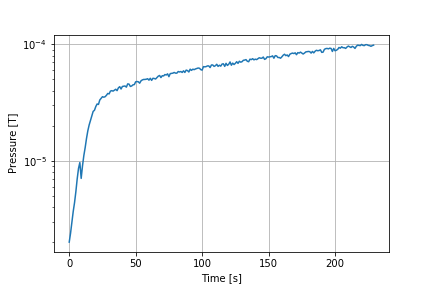
\includegraphics[width=\textwidth]{images/example.png}
    \caption{caption}
  \end{minipage}
  \hfill
  \begin{minipage}[b]{0.4\textwidth}
    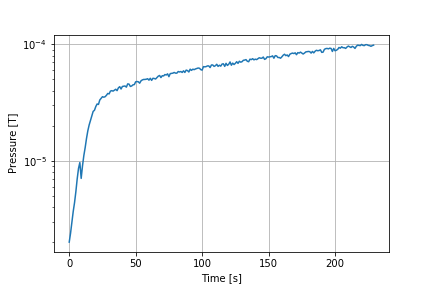
\includegraphics[width=\textwidth]{images/example.png}
    \caption{Caption}
  \end{minipage}
\end{figure}

\subsection{Raspberry Pi}
Content goes here

\newpage
% -----------------------------------Section 2----------------------------------------
\section{Section 2}
Subtitle

\subsection{Section}
Content goes here

\begin{itemize}
	\item \textbf{Listed} text
    \item \textbf{Listed} text
    \item \textbf{Listed} text
\end{itemize}

\subsection{Section}
Content goes here

\subsection{Section}
Content goes here

\subsubsection{Section}
Content goes here

\subsubsection{Section}
Content goes here

\subsubsection{Section}
Content goes here

\begin{figure}[ht]
  \centering
  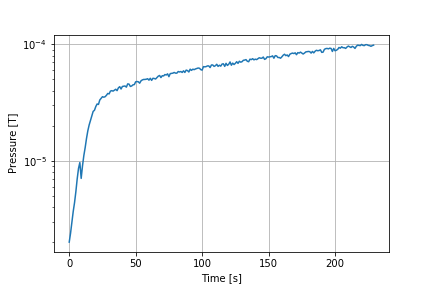
\includegraphics[height=7cm]{images/example.png}
  \caption{Caption}
\end{figure}

\subsubsection{Section}
Content goes here

\begin{scala}
code goes here
\end{scala}

\newpage
% -----------------------------------Section 3----------------------------------------

\section{Section 3}
\subsection{Section}
Content goes here

\subsection{Section}
Content goes here

\newpage
% -----------------------------------Appendix----------------------------------------
\section{Appendix}
\subsection{Appendix section}
Content goes here

\subsection{Appendix section}
Content goes here

\subsubsection*{Section not in table of contents}
Content goes here
\newpage
% -----------------------------------REFERENCE----------------------------------------
\begin{thebibliography}{9}
\bibitem{Erdos01} P. Erd\H os, \emph{A selection of problems and
results in combinatorics}, Recent trends in combinatorics (Matrahaza,
1995), Cambridge Univ. Press, Cambridge, 2001, pp. 1--6.
\end{thebibliography}
\end{document}

